\documentclass[10pt]{article}
\usepackage[utf8]{inputenc}
\usepackage[T1]{fontenc}
\usepackage{amsmath}
\usepackage{amsfonts}
\usepackage{amssymb}
\usepackage[version=4]{mhchem}
\usepackage{stmaryrd}
\usepackage{graphicx}
\usepackage[export]{adjustbox}
\graphicspath{ {./images/} }

\def\AA{\mathring{\mathrm{A}}}

\begin{document}
\section*{CHEMISTRY}
\section*{SECTION-A}
\begin{enumerate}
  \setcounter{enumi}{30}
  \item Which of the following reaction is correct?\\
(1) \(2 \mathrm{LiNO}_{3} \xrightarrow{\Delta} 2 \mathrm{LiNO}_{2}+\mathrm{O}_{2}\)\\
(2) \(4 \mathrm{LiNO}_{3} \xrightarrow{\Delta} 2 \mathrm{Li}_{2} \mathrm{O}+2 \mathrm{~N}_{2} \mathrm{O}_{4}+\mathrm{O}_{2}\)\\
(3) \(4 \mathrm{LiNO}_{3} \xrightarrow{\Delta} 2 \mathrm{Li}_{2} \mathrm{O}+4 \mathrm{NO}_{2}+\mathrm{O}_{2}\)\\
(4) \(2 \mathrm{LiNO}_{3} \xrightarrow{\Delta} 2 \mathrm{Li}+2 \mathrm{NO}_{2}+\mathrm{O}_{2}\)
\end{enumerate}

Official Ans. by NTA (3)\\
Allen Ans. (3)\\
Sol. \(\quad 4 \mathrm{LiNO}_{3} \xrightarrow{\Delta} 2 \mathrm{Li}_{2} \mathrm{O}+4 \mathrm{NO}_{2}+\mathrm{O}_{2}\)\\
32. The most stable carbocation for the following is:\\
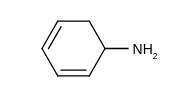
\includegraphics{smile-59ef2af8fad064e6af53d006174f41750c6eabbc}

(a)\\
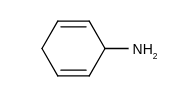
\includegraphics{smile-5ecbd2f8ec05bbe2fd4fd8b2f50e0aafefac042a}

(b)\\
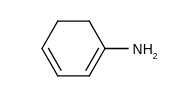
\includegraphics{smile-e434b2f4c29a873d8b62f238415360de2cd64928}

(c)\\
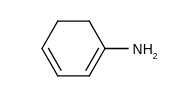
\includegraphics{smile-0ea3f8fa8ef6d3895db8013d97100f7a91828769}

(d)\\
(1) c\\
(2) d\\
(3) b\\
(4) a

Official Ans. by NTA (1)\\
Allen Ans. (1)

Sol.\\
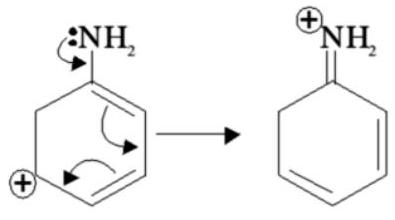
\includegraphics[max width=\textwidth, center]{2025_10_03_53db536d3401d6306e61g-1}

The +M effect of \(\mathrm{NH}_{2}\) is stabilizing the carbocation.\\
33. The correct order of \(\mathrm{pK}_{\mathrm{a}}\) values for the following compounds is:\\
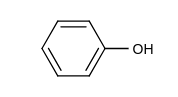
\includegraphics{smile-c48910f2c79df2b406b85626ee3d1cb941c030cc}

(a)\\
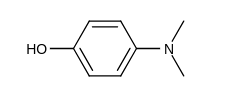
\includegraphics{smile-e496d68db10164756c125f2322f3dfc191942c41}

(b)\\
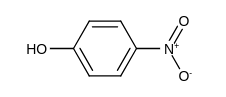
\includegraphics{smile-55592348f0ff23acfb2eef2b8f3fc5c4da73de9d}

(c)\\
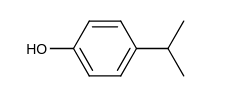
\includegraphics{smile-1213c42d9a93efda4aa69b8b4c8b4deb955f5ccd}

(d)\\
(1) \(c>a>d>b\)\\
(2) \(b>d>a>c\)\\
(3) \(b>a>d>c\)\\
(4) \(a>b>c>d\)

Official Ans. by NTA (2)\\
Allen Ans. (2)

\section*{TEST PAPER WITH SOLUTION}
Sol. Due to -M effect of \(-\mathrm{NO}_{2}\) group, it increases acidity +M effect of \(\mathrm{N}\left(\mathrm{CH}_{3}\right)_{2}\) decreases acidity.\\
Hyperconjugation of isopropyl decrease acidity\\
\(\therefore\) order of acidic strength\\
(c) \(>\) (a) \(>\) (d) \(>\) (b)\\
34. Decreasing order towards \(\mathrm{S}_{\mathrm{N}} 1\) reaction for the following compounds is:\\
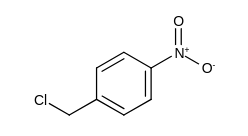
\includegraphics{smile-8d6270fee2bb3ef7b671b770f4f5ea1a1767ca39}

(a)\\
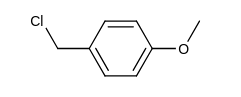
\includegraphics{smile-d844aeec111205e4505cd7cc03877f0118a98517}

(b)\\
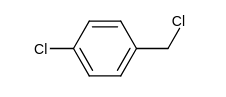
\includegraphics{smile-d5484c4376cfccf4dcad72898cb104a83f1c2e6b}

(c)\\
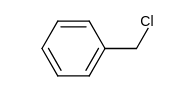
\includegraphics{smile-805bf876c181d8a938a0f45657deb45201987c6f}

(d)\\
(1) \(a>c>d>b\)\\
(2) \(a>b>c>d\)\\
(3) \(b>d>c>a\)\\
(4) \(d>b>c>a\)

Official Ans. by NTA (3)\\
Allen Ans. (3)\\
Sol. The rate of \(\mathrm{S}_{\mathrm{N}} 1\) reaction depends upon stability of carbocation which follows the order\\
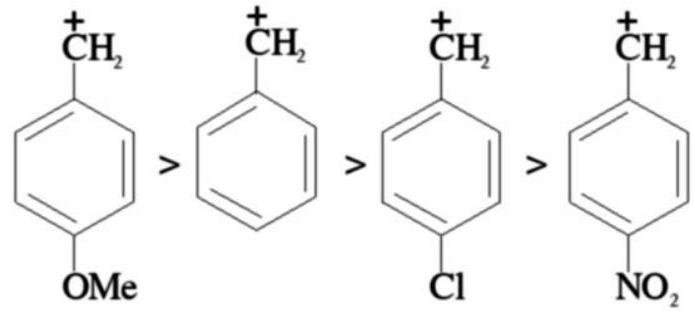
\includegraphics[max width=\textwidth, center]{2025_10_03_53db536d3401d6306e61g-1(1)}\\
\(\therefore\) Reactivity order\\
(b) \(>\) (d) \(>\) (c) \(>\) (a)\\
35.\\
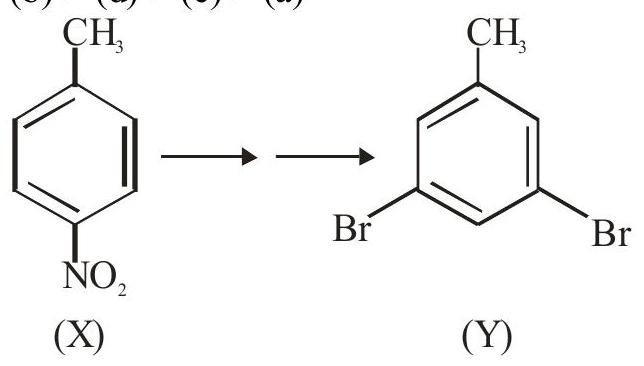
\includegraphics[max width=\textwidth, center]{2025_10_03_53db536d3401d6306e61g-1(2)}

In the above conversion of compound ( X ) to product (Y), the sequence of reagents to be used will be:\\
(1) (i) \(\mathrm{Br}_{2}, \mathrm{Fe}\)\\
(ii) \(\mathrm{Fe}, \mathrm{H}^{+}\)\\
(iii) \(\mathrm{LiAlH}_{4}\)\\
(2) (i) \(\mathrm{Br}_{2}(\mathrm{aq})\)\\
(ii) \(\mathrm{LiAlH}_{4}\) (iii) \(\mathrm{H}_{3} \mathrm{O}^{+}\)\\
(3) (i) \(\mathrm{Fe}, \mathrm{H}^{+}\)\\
(ii) \(\mathrm{Br}_{2}(\mathrm{aq})\)\\
(iii) \(\mathrm{HNO}_{2}\)\\
(iv) CuBr\\
(4) (i) \(\mathrm{Fe}, \mathrm{H}^{+}\)\\
(ii) \(\mathrm{Br}_{2}(\mathrm{aq})\)\\
(iii) \(\mathrm{HNO}_{2}\)\\
(iv) \(\mathrm{H}_{3} \mathrm{PO}_{2}\)

Official Ans. by NTA (4)\\
Allen Ans. (4)

Sol.\\
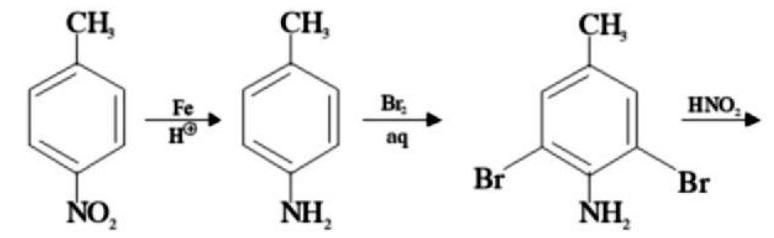
\includegraphics[max width=\textwidth, center]{2025_10_03_53db536d3401d6306e61g-2(2)}\\
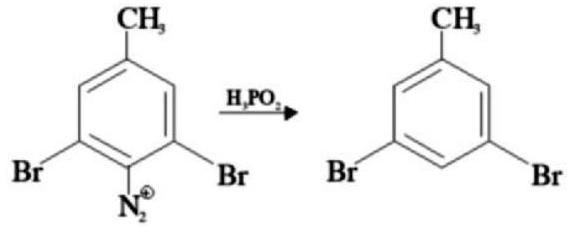
\includegraphics[max width=\textwidth, center]{2025_10_03_53db536d3401d6306e61g-2(1)}\\
36. Maximum number of electrons that can be accommodated in shell with \(\mathrm{n}=4\) are:\\
(1) 16\\
(2) 32\\
(3) 50\\
(4) 72

Official Ans. by NTA (2)\\
Allen Ans. (2)\\
Sol. The number of electrons in the orbitals of sub-shell of \(\mathrm{n}=4\) are

\begin{center}
\begin{tabular}{|c|r|}
\hline
4 s & 2 \\
\hline
4 p & 6 \\
\hline
4 d & 10 \\
\hline
4 f & 14 \\
\hline
(Total) & \(\mathbf{3 2}\) \\
\hline
\end{tabular}
\end{center}

\begin{enumerate}
  \setcounter{enumi}{36}
  \item Match List I with List II:
\end{enumerate}

\begin{center}
\begin{tabular}{|l|l|c|l|}
\hline
 & \multicolumn{1}{|c|}{\begin{tabular}{c}
List I \\
(Complexes) \\
\end{tabular}} &  & \multicolumn{1}{|c|}{\begin{tabular}{c}
List II \\
(Hybridisation) \\
\end{tabular}} \\
\hline
(A) & \(\left[\mathrm{Ni}(\mathrm{CO})_{4}\right]\) & I & \(\mathrm{sp}^{3}\) \\
\hline
(B) & \(\left[\mathrm{Cu}\left(\mathrm{NH}_{3}\right)_{4}\right]^{2+}\) & II & \(\mathrm{dsp}^{2}\) \\
\hline
(C) & \(\left[\mathrm{Fe}\left(\mathrm{NH}_{3}\right)_{6}\right]^{2+}\) & III & \(\mathrm{sp}^{3} \mathrm{~d}^{2}\) \\
\hline
(D) & \(\left[\mathrm{Fe}\left(\mathrm{H}_{2} \mathrm{O}\right)_{6}\right]^{2+}\) & IV & \(\mathrm{d}^{2} \mathrm{sp}^{3}\) \\
\hline
\end{tabular}
\end{center}

(1) \(\mathrm{A}-\mathrm{II}, \mathrm{B}-\mathrm{I}, \mathrm{C}-\mathrm{III}, \mathrm{D}-\mathrm{IV}\)\\
(2) \(\mathrm{A}-\mathrm{I}, \mathrm{B}-\mathrm{II}, \mathrm{C}-\mathrm{III}, \mathrm{D}-\mathrm{IV}\)\\
(3) \(\mathrm{A}-\mathrm{II}, \mathrm{B}-\mathrm{I}, \mathrm{C}-\mathrm{IV}, \mathrm{D}-\mathrm{III}\)\\
(4) A - I, B- II, C-IV, D-III

Official Ans. by NTA (4)\\
Allen Ans. (BONUS)\\
Sol. For \(\left[\mathrm{Fe}\left(\mathrm{NH}_{3}\right)_{6}\right]^{+2}, \Delta_{0}<\mathrm{P}\), hence the pairing of electrons does not occur in \(\mathrm{t}_{2 \mathrm{~g}}\). Therefore complex is outer orbital and its hybridisation is \(\mathrm{sp}^{3} \mathrm{~d}^{2}\).

\begin{center}
\begin{tabular}{|l|c|}
\hline
\multicolumn{1}{|c|}{\begin{tabular}{c}
List I \\
(Complexes) \\
\end{tabular}} & \begin{tabular}{c}
List II \\
(Hybridisation) \\
\end{tabular} \\
\hline
\(\left[\mathrm{Ni}(\mathrm{CO})_{4}\right]\) & \(\mathrm{sp}^{3}\) \\
\hline
\(\left[\mathrm{Cu}\left(\mathrm{NH}_{3}\right)_{4}\right]^{2+}\) & \(\mathrm{dsp}^{2}\) \\
\hline
\(\left[\mathrm{Fe}\left(\mathrm{NH}_{3}\right)_{6}\right]^{2+}\) & \(\mathrm{sp}^{3} \mathrm{~d}^{2}\) \\
\hline
\(\left[\mathrm{Fe}\left(\mathrm{H}_{2} \mathrm{O}\right)_{6}\right]^{2+}\) & \(\mathrm{sp}^{3} \mathrm{~d}^{2}\) \\
\hline
\end{tabular}
\end{center}

\begin{enumerate}
  \setcounter{enumi}{37}
  \item The \(\mathrm{Cl}-\mathrm{Co}-\mathrm{Cl}\) bond angle values in a fac\(\left[\mathrm{Co}\left(\mathrm{NH}_{3}\right)_{3} \mathrm{Cl}_{3}\right]\) complex is/are:\\
(1) \(90^{\circ} \& 180^{\circ}\)\\
(2) \(90^{\circ}\)\\
(3) \(180^{\circ}\)\\
(4) \(90^{\circ} \& 120^{\circ}\)
\end{enumerate}

Official Ans. by NTA (2)\\
Allen Ans. (2)

Sol.\\
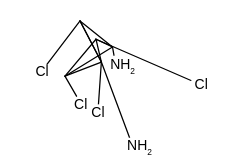
\includegraphics{smile-589000fd44eaa1a6d9196cf14ca339d254a6306b}

The \(\mathrm{Cl}-\mathrm{Co}-\mathrm{Cl}\) bond angle in above octahedral complex is \(90^{\circ}\)\\
39. Given below are two statements: One is labelled as Assertion A and the other is labelled as Reason R.

Assertion A :\\
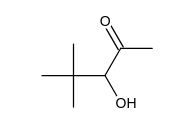
\includegraphics{smile-849d1ecce3b4b03a08dd92aa2645bd16a9fb10da}\\
can be easily reduced using \(\mathrm{Zn}-\mathrm{Hg} / \mathrm{HCl}\) to\\
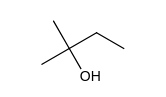
\includegraphics{smile-9b53cb128b930bbac2a4735a3f6d3e018698ccb7}

Reason \(\mathbf{R}: \mathrm{Zn}-\mathrm{Hg} / \mathrm{HCl}\) is used to reduce carbonyl group to \(-\mathrm{CH}_{2}-\) group.\\
In the light of the above statements, choose the correct answer from the options given below:\\
(1) A is false but R is true\\
(2) A is true but R is false\\
(3) Both A and R are true but R is not the correct explanation of A\\
(4) Both A and R are true and R is the correct explanation of A\\
Official Ans. by NTA (1)\\
Allen Ans. (1)

Sol.\\
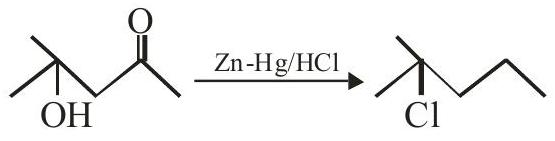
\includegraphics[max width=\textwidth, center]{2025_10_03_53db536d3401d6306e61g-2}

The acid sensitive alcohol group reacts with HCl , hence Clemmenson reduction is not suitable for above conversion.\\
40. Chlorides of which metal are soluble in organic solvents:\\
(1) Ca\\
(2) Mg\\
(3) K\\
(4) Be

Official Ans. by NTA (4)\\
Allen Ans. (4)\\
Sol. \(\mathrm{BeCl}_{2}\) having covalent nature is soluble in organic solvent.\\
41. Given below are two statements: One is labelled as Assertion A and the other labelled as Reason R.\\
Assertion A: Antihistamines do not affect the secretion of acid in stomach.\\
Reason R : Antiallergic and antacid drugs work on different receptors.\\
In the light of the above statements, choose the correct answer from the options given below:\\
(1) A is false but R is true\\
(2) Both A and R are true and R is the correct explanation of A\\
(3) A is true but R is false\\
(4) Both A and R are true but R is not the correct explanation of A .\\
Official Ans. by NTA (2)\\
Allen Ans. (2)\\
Sol. Antiallergic and antacid drugs work on different receptors\\
NCERT(XII) vol. 2 page no. 451-452\\
42. The wave function ( \(\Psi\) ) of 2 s is given by\\
\(\Psi_{2 s}=\frac{1}{2 \sqrt{2 \pi}}\left(\frac{1}{a_{0}}\right)^{1 / 2}\left(2-\frac{r}{a_{0}}\right) e^{-r / 2 a_{0}}\)\\
At \(r=r_{0}\), radial node is formed. Thus, \(r_{0}\) in terms of \(a_{0}\)\\
(1) \(r_{0}=a_{0}\)\\
(2) \(r_{0}=4 a_{0}\)\\
(3) \(\mathrm{r}_{0}=\frac{\mathrm{a}_{0}}{2}\)\\
(4) \(\mathrm{r}_{0}=2 \mathrm{a}_{0}\)

Official Ans. by NTA (4)\\
Allen Ans. (4)\\
Sol. At node \(\Psi_{2 \mathrm{~s}}=0\)\\
\(\therefore 2-\frac{\mathrm{r}_{0}}{\mathrm{a}_{0}}=0\)\\
\(\therefore \mathrm{r}_{0}=2 \mathrm{a}_{0}\)\\
43. \(\mathrm{KMnO}_{4}\) oxidises \(\mathrm{I}^{-}\)in acidic and neutral/faintly alkaline solution, respectively to\\
(1) \(\mathrm{I}_{2} \& \mathrm{IO}_{3}^{-}\)\\
(2) \(\mathrm{IO}_{3}^{-} \& \mathrm{I}_{2}\)\\
(3) \(\mathrm{IO}_{3}^{-} \& \mathrm{IO}_{3}^{-}\)\\
(4) \(\mathrm{I}_{2} \& \mathrm{I}_{2}\)

Official Ans. by NTA (1)\\
Allen Ans. (1)\\
Sol. In acidic medium\\
\(2 \mathrm{MnO}_{4}^{-}+10 \mathrm{I}^{-}+16 \mathrm{H}^{+} \rightarrow 2 \mathrm{Mn}^{2+}+5 \mathrm{I}_{2}+8 \mathrm{H}_{2} \mathrm{O}\)\\
In neutral/faintly alkaline solution\\
\(2 \mathrm{MnO}_{4}^{-}+\mathrm{I}^{-}+\mathrm{H}_{2} \mathrm{O} \rightarrow 2 \mathrm{MnO}_{2}+2 \mathrm{OH}^{-}+\mathrm{IO}_{3}^{-}\)\\
44. Bond dissociation energy of \(\mathrm{E}-\mathrm{H}\) bond of the " \(\mathrm{H}_{2} \mathrm{E}\) " hydrides of group 16 elements (given below), follows order.\\
(A) O\\
(B) S\\
(C) Se\\
(D) Te\\
(1) A \(>\) B \(>\) C \(>\) D\\
(2) \(\mathrm{A}>\mathrm{B}>\mathrm{D}>\mathrm{C}\)\\
(3) \(\mathrm{B}>\mathrm{A}>\mathrm{C}>\mathrm{D}\)\\
(4) \(\mathrm{D}>\mathrm{C}>\mathrm{B}>\mathrm{A}\)

Official Ans. by NTA (1)\\
Allen Ans. (1)\\
Sol. Bond dissociation energy of E-H bond in hydrides of group 16 follows the order\\
\(\mathrm{H}_{2} \mathrm{O}>\mathrm{H}_{2} \mathrm{~S}>\mathrm{H}_{2} \mathrm{Se}>\mathrm{H}_{2} \mathrm{Te}\)\\
45. The water quality of a pond was analysed and its BOD was found to be 4 . The pond has\\
(1) Highly polluted water\\
(2) Water has high amount of fluoride compounds\\
(3) Very clean water\\
(4) Slightly polluted water

Official Ans. by NTA (3)\\
Allen Ans. (3)\\
Sol. Clean water as BOD value of \(<5\) while polluted water has BOD of 15 or more.\\
46. Match List I with List II:

\begin{center}
\begin{tabular}{|l|l|l|l|}
\hline
 & List I (Mixture) &  & List II (Separation Technique) \\
\hline
(A) & \(\mathrm{CHCl}_{3}+\mathrm{C}_{6} \mathrm{H}_{5} \mathrm{NH}_{2}\) & I & Steam distillation \\
\hline
(B) & \(\mathrm{C}_{6} \mathrm{H}_{14}+\mathrm{C}_{5} \mathrm{H}_{12}\) & II & Differential extraction \\
\hline
(C) & \(\mathrm{C}_{6} \mathrm{H}_{5} \mathrm{NH}_{2}+\mathrm{H}_{2} \mathrm{O}\) & III & Distillation \\
\hline
(D) & Organic compound in \(\mathrm{H}_{2} \mathrm{O}\) & IV & Fractional distillation \\
\hline
\end{tabular}
\end{center}

(1) A-IV, B-I, C-III, D-II\\
(2) A-III, B-IV, C-I, D-II\\
(3) A-II, B-I, C-III, D-IV\\
(4) A-III, B-I, C-IV, D-II

Official Ans. by NTA (2)\\
Allen Ans. (2)\\
Sol.

\begin{center}
\begin{tabular}{|l|l|}
\hline
\multicolumn{1}{|c|}{List I (Mixture)} & \multicolumn{1}{|c|}{\begin{tabular}{c}
List II \\
(Separation \\
Technique) \\
\end{tabular}} \\
\hline
\(\mathrm{CHCl}_{3}+\mathrm{C}_{6} \mathrm{H}_{5} \mathrm{NH}_{2}\) & Distillation \\
\hline
\(\mathrm{C}_{6} \mathrm{H}_{14}+\mathrm{C}_{5} \mathrm{H}_{12}\) & \begin{tabular}{l}
Fractional \\
distillation \\
\end{tabular} \\
\hline
\(\mathrm{C}_{6} \mathrm{H}_{5} \mathrm{NH}_{2}+\mathrm{H}_{2} \mathrm{O}\) & Steam distillation \\
\hline
\begin{tabular}{l}
Organic compound \\
in \(\mathrm{H}_{2} \mathrm{O}\) \\
\end{tabular} & \begin{tabular}{l}
Differential \\
extraction \\
\end{tabular} \\
\hline
\end{tabular}
\end{center}

NCERT (XI) Vol. 2 Page No. 359, 360.\\
47. Boric acid in solid, whereas \(\mathrm{BF}_{3}\) is gas at room temperature because of\\
(1) Strong ionic bond in Boric acid\\
(2) Strong van der Waal's interaction in Boric acid\\
(3) Strong hydrogen bond in Boric acid\\
(4) Strong covalent bond in \(\mathrm{BF}_{3}\)

Official Ans. by NTA (3)\\
Allen Ans. (3)\\
Sol. Boric acid has strong hydrogen bonding while \(\mathrm{BF}_{3}\) does not. Therefore boric acid is solid.\\
48. Given below are two statements:

Statement I: During Electrolytic refining, the pure metal is made to act as anode and its impure metallic form is used as cathode.\\
Statement II: During the Hall-Heroult electrolysis process, purified \(\mathrm{Al}_{2} \mathrm{O}_{3}\) is mixed with \(\mathrm{Na}_{3} \mathrm{AlF}_{6}\) to lower the melting point of the mixture.\\
In the light of the above statements, choose the most appropriate answer from the options given below:\\
(1) Statement I is incorrect but Statement II is correct\\
(2) Both Statement I and Statement II are incorrect\\
(3) Statement I is correct but Statement II is incorrect\\
(4) Both Statement I and Statement II are correct

Official Ans. by NTA (1)\\
Allen Ans. (1)\\
Sol. In Electrolytic refining, the pure metal is used as cathode and impure metal is used as anode.\\
\(\mathrm{Na}_{3} \mathrm{AlF}_{6}\) is added during electrolysis of \(\mathrm{Al}_{2} \mathrm{O}_{3}\) to lower the melting point and increase conductivity.\\
49. Formulae for Nessler's reagent is:\\
(1) \(\mathrm{KHg}_{2} \mathrm{I}_{2}\)\\
(2) \(\mathrm{KHgI}_{3}\)\\
(3) \(\mathrm{K}_{2} \mathrm{HgI}_{4}\)\\
(4) \(\mathrm{HgI}_{2}\)

Official Ans. by NTA (3)\\
Allen Ans. (3)\\
Sol. Nessler's reagent is \(\mathrm{K}_{2} \mathrm{HgI}_{4}\).\\
50. \(1 \mathrm{~L}, 0.02 \mathrm{M}\) solution of \(\left[\mathrm{Co}\left(\mathrm{NH}_{3}\right)_{5} \mathrm{SO}_{4}\right] \mathrm{Br}\) is mixed with \(1 \mathrm{~L}, 0.02 \mathrm{M}\) solution of \(\left[\mathrm{Co}\left(\mathrm{NH}_{3}\right)_{5} \mathrm{Br}\right] \mathrm{SO}_{4}\). The resulting solution is divided into two equal parts \((\mathrm{X})\) and treated with excess \(\mathrm{AgNO}_{3}\) solution and \(\mathrm{BaCl}_{2}\) solution respectively as shown below:\\
1 L Solution \((\mathrm{X})+\mathrm{AgNO}_{3}\) solution (excess) \(\rightarrow \mathrm{Y}\)\\
1 L Solution ( X ) \(+\mathrm{BaCl}_{2}\) solution (excess) \(\rightarrow \mathrm{Z}\)\\
The number of moles of Y and Z respectively are\\
(1) \(0.02,0.02\)\\
(2) \(0.01,0.01\)\\
(3) \(0.02,0.01\)\\
(4) \(0.01,0.02\)

Official Ans. by NTA (2)\\
Allen Ans. (2)\\
Sol. \(\left[\mathrm{Co}\left(\mathrm{NH}_{3}\right)_{5} \mathrm{SO}_{4}\right] \mathrm{Br}+\mathrm{AgNO}_{3} \rightarrow \mathrm{AgBr} \downarrow 0.01 \mathrm{~mol} \quad\) excess \(\quad 0.01 \mathrm{Mol}\)\\
\(\left[\mathrm{Co}\left(\mathrm{NH}_{3}\right)_{5} \mathrm{Br}\right] \mathrm{SO}_{4}+\mathrm{BaCl}_{2} \rightarrow \mathrm{BaSO}_{4} \downarrow\) 0.01 mol excess 0.01 Mol

\section*{SECTION-B}
\begin{enumerate}
  \setcounter{enumi}{50}
  \item 1 mole of ideal gas is allowed to expand reversibly and adiabatically from a temperature of \(27^{\circ} \mathrm{C}\). The work done is \(3 \mathrm{~kJ} \mathrm{~mol}^{-1}\). The final temperature of the gas is \(\_\_\_\_\) K (Nearest integer). Given \(\mathrm{C}_{\mathrm{v}}=20 \mathrm{~J} \mathrm{~mol}^{-1} \mathrm{~K}^{-1}\).
\end{enumerate}

Official Ans. by NTA (150)\\
Allen Ans. (150)

Sol. \(\mathrm{q}=0\)\\
\(\Delta \mathrm{U}=\mathrm{w}\)\\
\(1 \times 20 \times\left[\mathrm{T}_{2}-300\right]=-3000\)\\
\(\mathrm{T}_{2}-300=-150\)\\
\(\mathrm{T}_{2}=150 \mathrm{~K}\)\\
52. Iron oxide FeO , crystallises in a cubic lattice with a unit cell edge length of \(5.0 \AA\). If density of the FeO in the crystal is \(4.0 \mathrm{~g} \mathrm{~cm}^{-3}\), then the number of FeO units present per unit cell is \(\_\_\_\_\) (Nearest integer)

Given : Molar mass of Fe and O is 56 and 16 g \(\mathrm{mol}^{-1}\) respectively.\\
\(\mathrm{N}_{\mathrm{A}}=6.0 \times 10^{23} \mathrm{~mol}^{-1}\)\\
Official Ans. by NTA (4)\\
Allen Ans. (4)\\
Sol. \(\quad d=\frac{Z \times M}{N_{0} \times a^{3}}\)\\
\(4=\frac{\mathrm{Z} \times 72}{6 \times 10^{23} \times 125 \times 10^{-24}}\)\\
\(Z=4.166 \simeq 4\)\\
53. An organic compound undergoes first order decomposition. If the time taken for the 60\% decomposition is 540 s , then the time required for \(90 \%\) decomposition will be is \(\_\_\_\_\) s. (Nearest integer).

Given : \(\ln 10=2.3 ; \log 2=0.3\)\\
Official Ans. by NTA (1350)

\section*{Allen Ans. (1350)}
Sol. \(\frac{\mathrm{t}_{1}}{\mathrm{t}_{2}}=\frac{\frac{1}{\mathrm{~K}} \ln \frac{\mathrm{a}_{0}}{0.4 \mathrm{a}_{0}}}{\frac{1}{\mathrm{~K}} \ln \frac{\mathrm{a}_{0}}{0.1 \mathrm{a}_{0}}}\)\\
\(\frac{540}{\mathrm{t}_{2}}=\frac{\ln \frac{10}{4}}{\ln 10}\)\\
\(\frac{540}{\mathrm{t}_{2}}=\frac{\log 10-\log 4}{\log 10}\)\\
\(\frac{540}{\mathrm{t}_{2}}=\frac{1-0.6}{1}\)\\
\(\Rightarrow \frac{540}{\mathrm{t}_{2}}=0.4\)\\
\(\Rightarrow \mathrm{t}_{2}=\frac{540}{0.4}=1350 \mathrm{sec}\)\\
54. Lead storage battery contains \(38 \%\) by weight solution of \(\mathrm{H}_{2} \mathrm{SO}_{4}\). The van't Hoff factor is 2.67 at this concentration. The temperature in Kelvin at which the solution in the battery will freeze is \(\_\_\_\_\)\\
(Nearest integer).\\
Given \(\mathrm{K}_{\mathrm{f}}=1.8 \mathrm{~K} \mathrm{~kg} \mathrm{~mol}^{-1}\)\\
Official Ans. by NTA (243)\\
Allen Ans. (243)\\
Sol. \(\quad \Delta \mathrm{T}_{\mathrm{f}}=\mathrm{i} . \mathrm{K}_{\mathrm{f}} . \mathrm{m}\)\\
\(\Rightarrow \Delta \mathrm{T}_{\mathrm{f}}=2.67 \times 1.8 \times \frac{38}{98} \times \frac{1000}{62}\)\\
\(\Rightarrow \Delta \mathrm{T}_{\mathrm{f}}=30.05\)\\
\(\therefore\) F.P. \(=243 \mathrm{~K}\)\\
55. Consider the following equation :\\
\(2 \mathrm{SO}_{2}(\mathrm{~g})+\mathrm{O}_{2}(\mathrm{~g}) \rightleftharpoons 2 \mathrm{SO}_{3}(\mathrm{~g}), \Delta \mathrm{H}=-190 \mathrm{~kJ}\)\\
The number of factors which will increase the yield of \(\mathrm{SO}_{3}\) at equilibrium from the following is\\
\(\_\_\_\_\)\\
A. Increasing temperature\\
B. Increasing pressure\\
C. Adding more \(\mathrm{SO}_{2}\)\\
D. Adding more \(\mathrm{O}_{2}\)\\
E. Addition of catalyst

Official Ans. by NTA (3)\\
Allen Ans. (3)\\
Sol. The yield of \(\mathrm{SO}_{3}\) at equilibrium will be due to :\\
B. Increasing pressure\\
C. Adding more \(\mathrm{SO}_{2}\)\\
D. Adding more \(\mathrm{O}_{2}\)\\
56. The graph of \(\log \frac{x}{m}\) vs \(\log p\) for an adsorption process is a straight line inclined at an angle of \(45^{\circ}\) with intercept equal to 0.6020 . The mass of gas adsorbed per unit mass of adsorbent at the pressure of 0.4 atm is \(\_\_\_\_\) \(\times 10^{-1}\) (Nearest integer)\\
Given : \(\log 2=0.3010\)\\
Official Ans. by NTA (16)\\
Allen Ans. (16)

Sol.\\
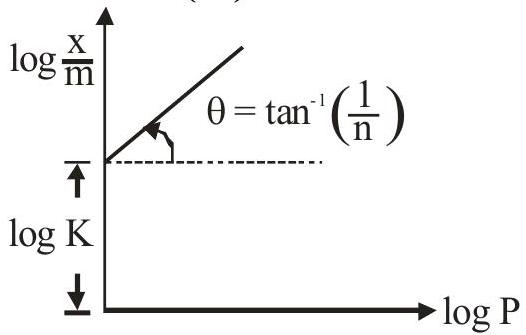
\includegraphics[max width=\textwidth, center]{2025_10_03_53db536d3401d6306e61g-6}\\
\(\log \frac{\mathrm{x}}{\mathrm{m}}=\log \mathrm{k}+\frac{1}{\mathrm{n}} \log \mathrm{P}\)\\
\(\frac{1}{\mathrm{n}}=\tan 45^{\circ}=1\)\\
\(\log \mathrm{k}=0.6020=\log 4\)\\
\(\Rightarrow \mathrm{K}=4\)\\
\(\therefore \frac{\mathrm{X}}{\mathrm{m}}=\mathrm{K} . \mathrm{P}^{1 / \mathrm{n}}\)\\
\(\frac{\mathrm{X}}{\mathrm{m}}=4(0.4)=1.6\)\\
\(\frac{\mathrm{x}}{\mathrm{m}}=1.6=16 \times 10^{-1}\)\\
57. Number of compounds from the following which will not dissolve in cold \(\mathrm{NaHCO}_{3}\) and NaOH solutions but will dissolve in hot NaOH solution is\\
\(\_\_\_\_\) .\\
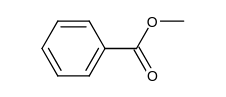
\includegraphics{smile-7f176c31c55811834971330cd2b5761d06ef33ab}\\
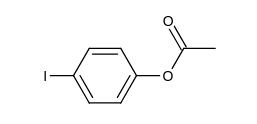
\includegraphics{smile-1a5d8d4e978350a0b83c4e4725cabfa2a3e9baeb}\\
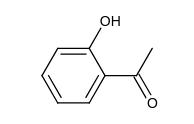
\includegraphics{smile-7dade3de1e845f775210324de25cb63b95bc7cb9}\\
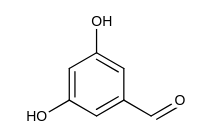
\includegraphics{smile-d111e87f41b5429d7fcdcba45c21c8c7e2b83cbd}

,\\
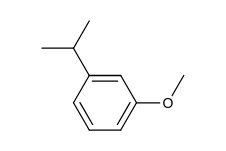
\includegraphics{smile-9b07b92d7a0fe59fd706881c31dd9ee2f4860f33}\\
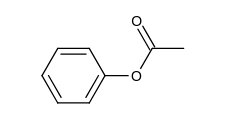
\includegraphics{smile-d9cad72c05449f8afdfde89517104870e11ba7aa}

Official Ans. by NTA (3)\\
Allen Ans. (3)\\
Sol. Compound 2, 3, 7\\
58. A short peptide on complete hydrolysis produces 3 moles of glycine (G), two moles of leucine (L) and two moles of valine ( V ) per mole of peptide. The number of peptide linkages in it are \(\_\_\_\_\) .

Official Ans. by NTA (6)\\
Allen Ans. (6)\\
Sol. Number of peptide linkage \(=(\) amino acid -1\()\)\\
\(=7-1=6\)\\
59. The strength of 50 volume solution of hydrogen peroxide is \(\_\_\_\_\) \(\mathrm{g} / \mathrm{L}\) (Nearest integer).

Given:\\
Molar mass of \(\mathrm{H}_{2} \mathrm{O}_{2}\) is \(34 \mathrm{~g} \mathrm{~mol}^{-1}\)\\
Molar volume of gas at \(\mathrm{STP}=22.7 \mathrm{~L}\).\\
Official Ans. by NTA (150)\\
Allen Ans. (150)\\
Sol. \(\quad\) Molarity \(=\frac{50}{11.35}\)\\
\(\therefore\) Strength in \(\mathrm{gm} / \mathrm{L}=\frac{50}{11.35} \times 34\)\\
60. The electrode potential of the following half cell at 298 K.\\
\(\mathrm{X}\left|\mathrm{X}^{2+}(0.001 \mathrm{M}) \| \mathrm{Y}^{2+}(0.01 \mathrm{M})\right| \mathrm{Y}\)\\
is \(\_\_\_\_\) \(\times 10^{-2} \mathrm{~V}\) (Nearest integer).

Given : \(\mathrm{E}_{\mathrm{x}^{2+} \mid \mathrm{x}}^{0}=-2.36 \mathrm{~V}\)\\
\(\mathrm{E}_{\mathrm{Y}^{2+} \mid \mathrm{Y}}^{0}=+0.36 \mathrm{~V}\)\\
\(\frac{2.303 \mathrm{RT}}{\mathrm{F}}=0.06 \mathrm{~V}\)\\
Official Ans. by NTA (275)\\
Allen Ans. (275)

Sol. \(\mathrm{X}+\mathrm{Y}^{2+} \rightarrow \mathrm{Y}+\mathrm{X}^{2+}\)

\begin{center}
\begin{tabular}{|l|}
\hline
\(\mathrm{E}_{\text {Cell }}^{0}=0.36-(-2.36)=2.72 \mathrm{~V}\) \\
\hline
\(\mathrm{E}_{\text {Cell }}=2.72-\frac{0.06}{2} \log \frac{0.001}{0.01}\) \\
\hline
\(=2.72+0.03=2.75 \mathrm{~V}\) \\
\hline
\(=275 \times 10^{-2} \mathrm{~V}\) \\
\hline
\end{tabular}
\end{center}


\end{document}